\begin{table}[t]

\centering
\begin{minipage}{0.575\textwidth}
\fontsize{8.45}{10.45}\selectfont
\begin{center}
\vspace{-0.8 cm}
\caption{\label{tab:inversion_vgg16} AR VGG-16 \cite{liu_2018_adv} feature inversion on ImageNet. Training our generator via pixel and feature losses, reconstruction largely improves by inverting AR representations.}
\begin{tabular}{c|c|c}
\specialrule{.15em}{.05em}{.05em} 
 & Standard Model & AR Model (ours)\\
 \hline
\makecell{Standard Accuracy} & $65.0$ & $48.7$\\
\makecell{$\ell_{\infty}$ PGD Accuracy} & $0$ & $23.0$\\
\hline
\makecell{PSNR (dB) $\uparrow$} & $18.35\pm 2.471$ & $\mathbf{21.063\pm 3.132}$\\
\makecell{SSIM $\uparrow$} & $0.466\pm 0.2$ & $\mathbf{0.538\pm 0.165}$\\
\makecell{LPIPS $\downarrow$} & $0.327\pm 0.101$ & $\mathbf{0.225\pm0.057}$\\
\specialrule{.15em}{.05em}{.05em} 
\end{tabular}
\end{center}
\end{minipage}
\hfill
\begin{minipage}{0.375\textwidth}
\hspace{2.21\baselineskip}\noindent\fcolorbox{white}{white}{\begin{minipage}[t]{0.155\textwidth}
\centering\textbf{{\scalebox{0.525}{\hspace{-0.25\baselineskip}G. truth}}}
\end{minipage}}\noindent\fcolorbox{white}{white}{\begin{minipage}[t]{0.16\textwidth}
\centering\textbf{{\scalebox{0.525}{\hspace{-0.15\baselineskip}Standard}}}
\end{minipage}}\noindent\fcolorbox{white}{white}{\begin{minipage}[t]{0.15\textwidth}
\centering\textbf{{\scalebox{0.525}{\hspace{-0.55\baselineskip}AR (Ours)}}}
\end{minipage}}

\begin{center}
\vspace{-0.475cm}
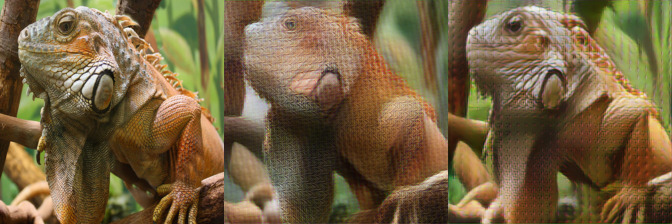
\includegraphics[width=0.63\textwidth]{figs/vgg16/rec_tile_0.jpg}

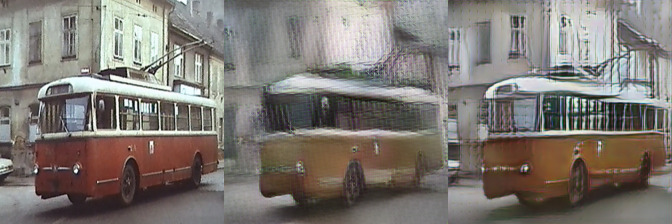
\includegraphics[width=0.63\textwidth]{figs/vgg16/rec_tile_1.jpg}

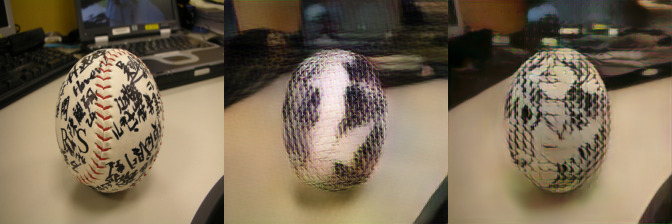
\includegraphics[width=0.63\textwidth]{figs/vgg16/rec_tile_2.jpg}
\end{center}
\captionof{figure}{\label{fig:inversion_vgg16} AR VGG-16 reconstruction on ImageNet.}
\end{minipage}
\vspace{-0.8 cm}
\end{table}
